% {{{ Preamble ----------------------------------------------------------------
\documentclass[a4paper,11pt]{article}

% encodings, fonts etc.
\usepackage[utf8]{inputenc}
\usepackage[T1]{fontenc}

% page layout
%\usepackage{a4wide}

% math packages
\usepackage{amsmath, amssymb, amsthm}
\usepackage{mathtools}

% graphics, colors, figures etc.
\usepackage{graphicx}
\usepackage{caption}
\usepackage{subcaption}
\usepackage{float}
\usepackage[export]{adjustbox}
\usepackage{color}



% misc. packages
\usepackage{hyperref}
\usepackage{url}
\usepackage{fancyvrb}

% code etc.
\usepackage{listings}

\usepackage{verbatim}
\usepackage[table,xcdraw]{xcolor}

\definecolor{mygreen}{rgb}{0,0.6,0}
\definecolor{mygray}{rgb}{0.5,0.5,0.5}
\definecolor{mymauve}{rgb}{0.58,0,0.82}

\lstset{%
  backgroundcolor=\color{white},
  basicstyle=\footnotesize\ttfamily,
  breakatwhitespace=true,
  breaklines=true,
  captionpos=t,
  commentstyle=\color{mygreen},
  extendedchars=true,
  keepspaces=true,
  keywordstyle=\color{blue},
  numbers=none,
  numbersep=8pt,
  numberstyle=\tiny\color{mygray},
  rulecolor=\color{black},
  showstringspaces=false,
  showtabs=false,
  stepnumber=1,
  stringstyle=\color{mymauve},
  frame=single,
  frameround=tttt,
  %frame=tb,
  belowskip=-0.2\baselineskip,
}

% mathematics, theorems etc.
\newtheorem*{proposition}{Proposition}
\newtheorem*{lemma}{Lemma}
\newtheorem*{theorem}{Theorem}
\newtheorem{example}{Example}
\theoremstyle{definition}
\newtheorem{definition}{Definition}[section]

% change \qed symbol to black square
\renewcommand\qedsymbol{$\blacksquare$}

% various useful commands
\newcommand{\file}[1]{\texttt{#1}}
\DeclareMathOperator*{\argmin}{arg\,min}
\def\LRA{\hspace{1em}\Leftrightarrow\hspace{1em}}

\newcommand{\type}[1]{\texttt{#1}}
\newcommand{\fun}[1]{\texttt{#1}}

\newcommand{\sfm}{\texttt{scan\_for\_matches}}


% tikz
\usepackage{pgf}
\usepackage{tikz}
\usetikzlibrary{arrows,automata,positioning}

% title page
\title{Kleenex-based approximate pattern matching for DNA analysis}
\author{Anders Kiel Hovgaard \and Daniel Lundberg Pedersen \and Dandan Xue}
\date{January 23, 2017}
% }}} -------------------------------------------------------------------------

\begin{document}

\maketitle

\begin{abstract}
  TODO: Write \dots
\end{abstract}
\newpage

\tableofcontents
\newpage

\section{Introduction}

Approximate pattern matching is the problem of finding occurrences of a given
pattern string in a given text string, while allowing some degree of error in
the occurrences. In other words, given some distance metric, the problem is to
find all the occurrences of the pattern in the text including those within a
specified distance of the pattern string. The pattern may denote a single
string, or a set of strings as in the case of a regular expression.

The problem is also known as approximate string matching or searching,
approximate regular string matching, approximate regular substring matching
etc. It is an important problem in many areas, including in bioinformatics
where common tasks involve searching for specific patterns in biological
sequences such as DNA, RNA, and protein, represented as text strings. However
these sequences may contain errors, thus presenting a need for approximate
search techniques.

A number of bachelor theses investigated the use of automata-based techniques
for DNA pattern matching and they compared their implementations to the widely
used domain-specific tool \sfm{}.  This turned out to be just barely
competitive with \sfm{} in some cases. Even more recently, the Kleenex language
and compiler~\cite{grathwohl2016kleenex,soholm2015ordered} was extended to
support approximate matching, and in fact approximate transduction, through
rewriting of core Kleenex programs to express approximate matching as exact
matching~\cite{troelsen2016approximate}. This has indicated even better
performance and even managed to outperform \sfm{} in one case. The evaluation
of this tool with regards to the application of approximate pattern matching in
biological sequences has, however, only been briefly investigated.

This project is about investigating the applicability of Kleenex to the topic
discussed above and comparing it to the NR-grep~\cite{navarro2001nr} program as
well as \sfm{}.

We have found that approximate Kleenex shows a competitive runtime performance
in many case, however often slightly outperformed by NR-grep, and while it is
sometimes outperforming \sfm{}, it does not seem to scale as well with increasing
number of allowed errors $k$. We have also found that the size of the program
generated by approximate Kleenex grows very large as $k$ increases, which is
possibly a major cause of performance degradation.

We also review other existing solutions to the problem of approximate matching
and we discuss potential improvements to the approximate Kleenex program.

%%% Local Variables:
%%% mode: latex
%%% TeX-master: "main"
%%% End:

\section{Background}

This section describes the main background theory of the Kleenex language and
its application to approximate string matching.

\subsection{Transducers}

Kleenex is a domain-specific language for expressing transducers. The concept
of a transducer extends that of a finite automaton to also include output, that
is, a finite automaton either accepts or rejects a string, whereas a transducer
produces an output string in a language over a given output alphabet.

First we define the notion of a finite state transducer, which is essentially
just a nondeterministic finite automaton (NFA) which can also output a symbol
on each transition.

\begin{definition}[FST]
  A \emph{finite state transducer} $\mathcal{T}$ over an input alphabet
  $\Sigma$ and an output alphabet $\Gamma$ is a structure
  $(\Sigma, \Gamma, Q, q^s, q^f, \Delta)$, where
  \begin{itemize}
      \item $Q$ is a finite set of states,
      \item $q^s, q^f \in Q$ are the initial and final states,
        respectively, and
      \item $\Delta \subseteq Q \times \Sigma[\epsilon] \times
        \Gamma[\epsilon] \times Q$ is the transition relation.
  \end{itemize}
\end{definition}

Here, $\Sigma[\epsilon]$ denotes the alphabet $\Sigma$ extended with the empty
string $\epsilon$.

Intuitively, there is the following correspondence between the elements of the
transition relation and the transitions in the drawn diagram of the transducer:
\[
  (q, s, t, q') \in \Delta \quad \Leftrightarrow \quad q \xrightarrow{s/t} q'
\]

In an NFA, multiple paths may lead to an accepting state for a given input
string, but regardsless of which accepting path is chosen, the ouput is the
same. In an FST, on the other hand, the path determines the transduced output,
thus the same input string may produce entirely different outputs depending on
the path chosen.

In order to disambiguate between different transductions of the same input
string, we introduce the notion of a normalized FST. To facilitate this, we
also introduce two new symbols $\epsilon_0$ and $\epsilon_1$. Both denote the
empty string, but they serve to distinguish between nondeterministic
$\epsilon$-transitions.

\begin{definition}[NFST]
  A \emph{normalized finite state transducer} is a deterministic FST,
  $T = (\Sigma[\epsilon_0,\epsilon_1], \Gamma, q^s, q^f, \Delta)$, with the
  constraint that $\forall q \in Q$, $q$ is either a choice state, a skip
  state, a symbol state, or the final state.
\end{definition}

The notions of choice, skip, or symbol states are perhaps best conveyed by
illustration, as shown in Figure~\ref{fig:nfst-states}.

\begin{figure}[!ht]
  \centering
  \begin{subfigure}[b]{0.3\textwidth}
    \centering
    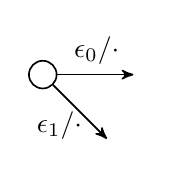
\begin{tikzpicture}[->,>=stealth',shorten >=1pt,auto,node distance=1.0cm,
      semithick, main/.style={circle,draw,minimum width=10pt}]
        \node[main] (q0) {$ $};
        \node       (q1) [right = of q0] {};
        \node       (q2) [below right = of q0] {};
        \path (q0) edge node {$\epsilon_0/\cdot$} (q1)
              (q0) edge node [below left = -2mm, swap]
                   {$\epsilon_1/\cdot$} (q2);
    \end{tikzpicture}
    \caption{A choice state.}
  \end{subfigure}
  ~
  \begin{subfigure}[b]{0.3\textwidth}
    \centering
    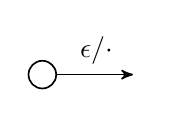
\begin{tikzpicture}[->,>=stealth',shorten >=1pt,auto,node distance=1.0cm,
        semithick, main/.style={circle,draw,minimum width=10pt}]
        \node[main] (q0) {$ $};
        \node       (q1) [right = of q0] {};
        \path (q0) edge node        {$\epsilon/\cdot$} (q1);
    \end{tikzpicture}
    \caption{A skip state.}
  \end{subfigure}
  ~
  \begin{subfigure}[b]{0.3\textwidth}
    \centering
    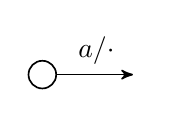
\begin{tikzpicture}[->,>=stealth',shorten >=1pt,auto,node distance=1.0cm,
      semithick, main/.style={circle,draw,minimum width=10pt}]
        \node[main] (q0) {$ $};
        \node       (q1) [right = of q0] {};
        \path (q0) edge node {$a/\cdot$} (q1);
    \end{tikzpicture}
    \caption{A symbol state.}
  \end{subfigure}
  \caption{Illustration of choice states, skip states, and symbol states.}
  \label{fig:nfst-states}
\end{figure}

Thus, the set of symbols that any state has transitions on, i.e. the support of
the state, is either just $\epsilon$, exactly $\{\epsilon_0, \epsilon_1\}$,
exactly one $a \in \Sigma$, or $\emptyset$ in the case of the final
state. % Therefore, an NFST is deterministic...





%%% Local Variables:
%%% mode: latex
%%% TeX-master: "main"
%%% End:

\section{Experiments}

\subsection{Introduction to the tools}


\subsection{Experiment setup and benchmark description}
The experiments where run on the \texttt{gpu02} machine
\begin{description}
    \item[CPU] Intel Xeon E5-2650 v2 (2.60 GHz)
    \item[RAM] 128 GB
\end{description}

The data set used for the benchmark is from
\url{ftp://ftp-trace.ncbi.nih.gov/1000genomes/ftp/technical/reference/human_g1k_v37.fasta.gz}
and is 2.9 GBs uncompressed, for most of the benchmarks we used a file where we
stripped the newlines, so they would not count as an error, except for the
nrgrep trails since it could not handle long lines.


\subsection{Results}


\section{Survey of approximate matching techniques}
Approximate matching is in general more complicated than exact matching. We can consider exact matching problems as a subset of approximate matching problems with an error of 0. The problem set will also change a lot if we use a different definition of the error metric or the type of errors. The time complexity of many efficient exact matching algorithms that work as simulating a DFA, such as the Knuth–Morris–Pratt algorithm, will become exponential as the number of errors grows if we just convert the NFA of the pattern into a DFA to be adapted in these algorithms. 

\begin{comment}

\subsection{Dynamic programming}

One of the classical solutions to approximate matching problem is to use dynamic programming. This method is simple and easy to be implemented by programming. 

% TODO: some examples maybe


\subsection{Autamata simulation}
Another classical one is automata simulation. The algortihm BNDM  (we will explain later) over which NR-grep is built is basically a simulation of an NFA. 

\end{comment}


\subsection{NR-grep}

\subsubsection{Bit-parallelism}
From the experiment results shown in the previous section, we can say in general NR-grep has the best performance in average in our various test cases. This is not surprising because NR-grep implemented different efficient algorithms for various pattern matching problems as well as a good software design. From this tool's perspective, the patterns are classified into three levels: simple patterns, extended patterns and regular experssions. Different algorithms are applied to different levels of patterns to make sure that the problem can be solved in the most efficient way. 

We now show the idea of how NR-grep solves the approximate matching in an efficient way. The name of this tool comes from "nondeterministic reverse $grep$", which indicates this tool can simulate NFAs instead of converting them to DFAs. The algorithm of  simulating NFAs used in NR-grep is called $Shift-Or$. This algorithm is based on an approach called $bit-parallelism$, which takes advantage of the parallelism of the bit operations inside a computer word. A variant of Shift-Or that is easier to explain is $Shift-And$ algorithm, which also based on $bit-parallelism$. We first show how this algorithm works. 

Given a pattern $pat$ of length $m$,  and a text $txt$ of length $n$ and the alphabet set is $\Sigma$ with a size $|\Sigma|$. First we build a table $B$ in which for each character in $\Sigma$ stores a bit mask $b_m...b_1$. Each bit mask in the table has a length of $m$. For a character $char$ in $pat$ with an index $i$ (1-indexed), set the $m-i-1$ bit of the mask in B[$char$]. The following example shows a bit mask table for the pattern "abc" assuming $\Sigma$ = {a,b,c,d}.


\begin{example}\emph{The bit mask table for pattern "abc".}

\begin{table}[H]
	\centering
	\begin{tabular}{|c|c|c|c|}
		\hline
		index      & 1                        & 2                        & 3                        \\ \hline
		\textbf{a} & 0                        & 0                        & {\color[HTML]{3531FF} 1} \\ \hline
		\textbf{b} & 0                        & {\color[HTML]{3531FF} 1} & 0                        \\ \hline
		\textbf{c} & {\color[HTML]{3531FF} 1} & 0                        & 0                        \\ \hline
		\textbf{d} & 0                        & 0                        & 0                        \\ \hline
	\end{tabular}
	\label{table-bitmask}
\end{table}
\end{example}

We use a computer word $D = d_m...d_1$ to store the current active state with an initial value of all bits 0. During the searching process, $D$ is updated with the following formula: 
$$D' \leftarrow ((D << 1) \ | \ 0^{m-1}1) \ \& \ B[t_j]$$
where $t_j$ is the next text character.  When the $d_m$ bit in $D$ is set, we report the match. 

One of the advantages of the $Shift-Or$ algorithm is that it is easy to be extended to handle classes of characters, which is helpful for approximate matching. 
For example, we can now search for the pattern "ab."\footnote{ We use symbol '.' in this report to stand for a wildcard.}, which can be considered as the pattern "abc" allows a replacement error at the third character by just setting the $m-3+1$ bit of all the characters in the bit mask table as the following example shows. 

\begin{example}\emph{The bit mask table for pattern "ab."}.
	\begin{table}[H]
		\centering
		\begin{tabular}{|c|c|c|c|}
			\hline
			index      & 1                        & 2                        & 3                        \\ \hline
			\textbf{a} & {\color{red} 1}                   & 0                        & {\color[HTML]{3531FF} 1} \\ \hline
			\textbf{b} &  {\color{red} 1}                    & {\color[HTML]{3531FF} 1} & 0                        \\ \hline
			\textbf{c} & {\color[HTML]{3531FF} 1} & 0                        & 0                        \\ \hline
			\textbf{d} &{\color{red} 1}                    & 0                        & 0                        \\ \hline
		\end{tabular}
		\label{table-bitmask2}
	\end{table}
\end{example}

With this new bit mask table, searching for the pattern "ab.", or more generally a pattern that contains wildcards, will be just the same time complexity as search for "abc". 
%We can also find that an error of insertion can be dealt with by adding a new row of all 1s in the bit mask table and a deletion is just removing one row. 
 
\subsubsection{BNDM algorithm}
As we know, many efficient pattern matching algorithms, such as the Knuth–Morris–Pratt and the Boyer-Moore algorithm, employ a trick of skipping characters. It is possible to combine the $bit-parallelism$ approach with the ability of skipping characters to achieve an even more efficient algorithm. This idea is implemented by the $BNDM$ algorithm, which is used in NR-grep. BNDM uses $Shift-Or$ instead of $Shift-And$, a variant of $Shift-And$ that uses the following state updating formula:  
$$ D' \leftarrow  (D \ \& \ B[t_j]) << 1 .$$ The algorithm that is adapted in BNDM for skipping charaters is from the Boyer-Moore or the BDM families\cite{crochemore1994text}.


\subsubsection{NFA simulation}
As we have shown above, bit-parallelism deals with single error efficiently.
Now we present how bit-parallelism can be used to simulate an NFA for approximate matching. 

Consider the pattern "ab" allowing one error, we can build an NFA to simulate it as the follow figure shows.

\begin{figure} [H]
\begin{center}
	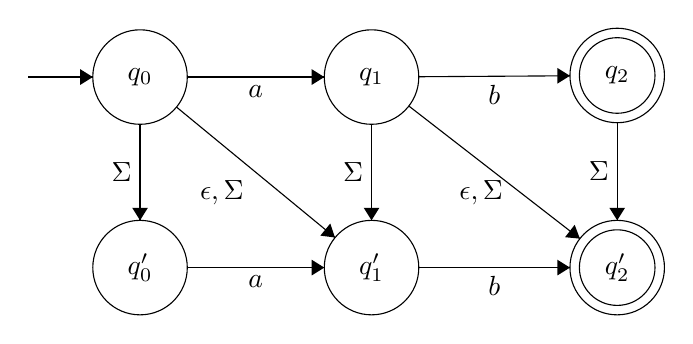
\begin{tikzpicture}[scale=0.2]
	\tikzstyle{every node}+=[inner sep=0pt]
	\draw [black] (18.3,-25.8) circle (3);
	\draw (18.3,-25.8) node {$q_0$};
	\draw [black] (33,-25.8) circle (3);
	\draw (33,-25.8) node {$q_1$};
	\draw [black] (18.3,-37.9) circle (3);
	\draw (18.3,-37.9) node {$q_0'$};
	\draw [black] (33,-37.9) circle (3);
	\draw (33,-37.9) node {$q_1'$};
	\draw [black] (48.6,-25.7) circle (3);
	\draw (48.6,-25.7) node {$q_2$};
	\draw [black] (48.6,-25.7) circle (2.4);
	\draw [black] (48.6,-37.9) circle (3);
	\draw (48.6,-37.9) node {$q_2'$};
	\draw [black] (48.6,-37.9) circle (2.4);
	\draw [black] (11.2,-25.8) -- (15.3,-25.8);
	\fill [black] (15.3,-25.8) -- (14.5,-25.3) -- (14.5,-26.3);
	\draw [black] (21.3,-25.8) -- (30,-25.8);
	\fill [black] (30,-25.8) -- (29.2,-25.3) -- (29.2,-26.3);
	\draw (25.65,-26.3) node [below] {$a$};
	\draw [black] (21.3,-37.9) -- (30,-37.9);
	\fill [black] (30,-37.9) -- (29.2,-37.4) -- (29.2,-38.4);
	\draw (25.65,-38.4) node [below] {$a$};
	\draw [black] (18.3,-28.8) -- (18.3,-34.9);
	\fill [black] (18.3,-34.9) -- (18.8,-34.1) -- (17.8,-34.1);
	\draw (17.8,-31.85) node [left] {$\Sigma$};
	\draw [black] (33,-28.8) -- (33,-34.9);
	\fill [black] (33,-34.9) -- (33.5,-34.1) -- (32.5,-34.1);
	\draw (32.5,-31.85) node [left] {$\Sigma$};
	\draw [black] (36,-25.78) -- (45.6,-25.72);
	\fill [black] (45.6,-25.72) -- (44.8,-25.22) -- (44.8,-26.22);
	\draw (40.8,-26.26) node [below] {$b$};
	\draw [black] (36,-37.9) -- (45.6,-37.9);
	\fill [black] (45.6,-37.9) -- (44.8,-37.4) -- (44.8,-38.4);
	\draw (40.8,-38.4) node [below] {$b$};
	\draw [black] (20.62,-27.71) -- (30.68,-35.99);
	\fill [black] (30.68,-35.99) -- (30.38,-35.1) -- (29.75,-35.87);
	\draw (23.49,-32.34) node [below] {$\epsilon, \Sigma$};
	\draw [black] (48.6,-28.7) -- (48.6,-34.9);
	\fill [black] (48.6,-34.9) -- (49.1,-34.1) -- (48.1,-34.1);
	\draw (48.1,-31.8) node [left] {$\Sigma$};
	\draw [black] (35.37,-27.64) -- (46.23,-36.06);
	\fill [black] (46.23,-36.06) -- (45.9,-35.18) -- (45.29,-35.97);
	\draw (39.96,-32.35) node [below] {$ \epsilon,\Sigma$};
	\end{tikzpicture}
\end{center}
\caption{An NFA accepting the pattern "ab" with at most one error. The label $\epsilon,\Sigma$ on the diagnoal arrows means both $\epsilon$ and $\Sigma$ can be accepted.}
\label{fig:nfa"ab"}
\end{figure}
 
In Figure \ref{fig:nfa"ab"}, the last state of each row stands for a state that accepts $r$ errors where $r$ is the index of the row (0-indexed). That is, in our example, the state $q_2$ accepts "ab" with no error and $q_2'$  with exact one error. The vertical arrows represent an insertion, and the $\epsilon$ and $\Sigma$ on the diagonal arrows stand for a deletion and a replacement respectively. We can image that we could build an NFA for any other patterns with $k$ errors in such manner iteratively. It is worth noting that the number of states in the NAF built in such a way increases linearly with the number of errors.

The technique stores each row in a machine word, say $R_i$ for row $i$ %just as we have shown in $Shift-And$.???
The updating of these words are performed with the following formulars: 

\begin{align*}
R_0' \leftarrow & ((R_0 << 1) \ |\ 0^{m-1}) \ \& \ B[t_j] \\
for \ &i \in 1...k \ do:  \\
	& R_i' \leftarrow ((R_i << 1) \ \& \ B[t_j] ) \ |\ R_{i-1} \ | \ (R_{i-1} << 1 ) \ |\ (R_{i-1}' << 1)
\end{align*}

These formulars show us one case of how bit-parallelism simulate an NFA. $R_0'$ is updated just as we have shown in $Shift-And$. In the formular for updating $R_i'$, the first element (i.e., $((R_i << 1) \ \& \ B[t_j] ) $ ) is similar to $Shitf-And$ but removed the OR operation with $O^{m-1}$ because it can not be an initial state that has a self-loop. The second is the old value of its upper row, which corresponds to a vertial arrow. Similarly, the third stands for a replacement and the fourth a deletion. When we detect that $R_k \& 10^{m-1}$ is set, a match is reported.  

As we can see from the above updating formulas, each updating is just bitwise operation hence constant time. So this simulation should be linear time complexity with $k$.
 
\subsection{Python (\texttt{regex})}

\subsection{Scan For Matches}


\subsection{Approximate Kleenex}
\section{Problem analysis}

\subsection{Analysis of automata generated by approximate kleenex}

Visualization.

\subsection{Improving kleenex}

% Counters, implemented as optimization in the implementation vs. updating the
% automata models.

In his bachelor's thesis~\cite{enevoldsen2015pattern}, Sune Enevoldsen uses the
concept of a tagged automaton, based on work by Ville
Laurikari~\cite{laurikari2000nfas, laurikari2001efficient} and inspired by
Levenshtein automata~\cite{schulz2002fast}, to do approximate regular string
matching.

A tagged NFA is an NFA extended with a set of tags which may be set or modified
on each transition in the transition relation. The idea is to use these tags as
counters which keep track of the allowed number of errors, e.g.  insertions,
deletion, and substitutions.

% Thus, the tagged automata for a given regular expression $RE$ will accept the
% strings in $\mathcal{L}(RE)$ as well as any string that is within a certain
% error distance of a string in $\mathcal{L}(RE)$.






%%% Local Variables:
%%% mode: latex
%%% TeX-master: "main"
%%% End:

\section{Conclusion}
As long as the patterns are simple enough so that Kleenex compiles a not too
large executable, it seems to be able to compete with or outperform the other
tools we have tested, with NR-grep being the biggest difference, but it does
have an unfair advantage in using the input with newlines.


\clearpage
\bibliographystyle{plain}
\bibliography{tipl}

\clearpage
\appendix
\section{Example of transducer for approximate Kleenex program}
\label{app:approx-kleenex-example}

\begin{figure}[!ht]
  \begin{subfigure}[t]{1\textwidth}
    \centering
    \includegraphics[width=0.5\textwidth]{images/as_exact.pdf}
    \caption{Transducer for the original program.}
  \end{subfigure}
  ~
  \noindent\makebox[\textwidth]{%
  \begin{subfigure}[t]{1.4\textwidth}
    \centering
    \includegraphics[width=\textwidth]{images/as_k2_hamming.pdf}
    \caption{Transducer for the rewritten program.}
  \end{subfigure}}
  \caption{Visualization of transducers for the original Kleenex program
    accepting exactly $a^*$ and the rewritten program accepting $a^*$ with
    $k=2$ errors using Hamming distance.}
\end{figure}

%%% Local Variables:
%%% mode: latex
%%% TeX-master: "main"
%%% End:


\end{document}

%%% Local Variables:
%%% mode: latex
%%% TeX-master: t
%%% End:
